% !TEX root =  ../report.tex
\section{Introduction}

\subsection{Evaluation objective}
The target group of the product consists of teams, from any field, that want to coordinate a collaborative effort. These people might not necessarily be tech-savvy and should preferably be able to use the product and all its core features without having to sift through a lengthy documentation or tutorial. As such, ease-of-use and an intuitive interface were highly prioritised by Group 22, the developers of "Unruly Guitar". The main goal of the evaluation was to amend any flaws that would compromise this by analysing the report and translating it to concrete goals that would be added to the backlog of the developers. 

\subsection{Prototype}

The product in question consists mainly of a board overview screen, where users can organise tasks, represented as "cards", into lists.

\begin{figure}[ht]
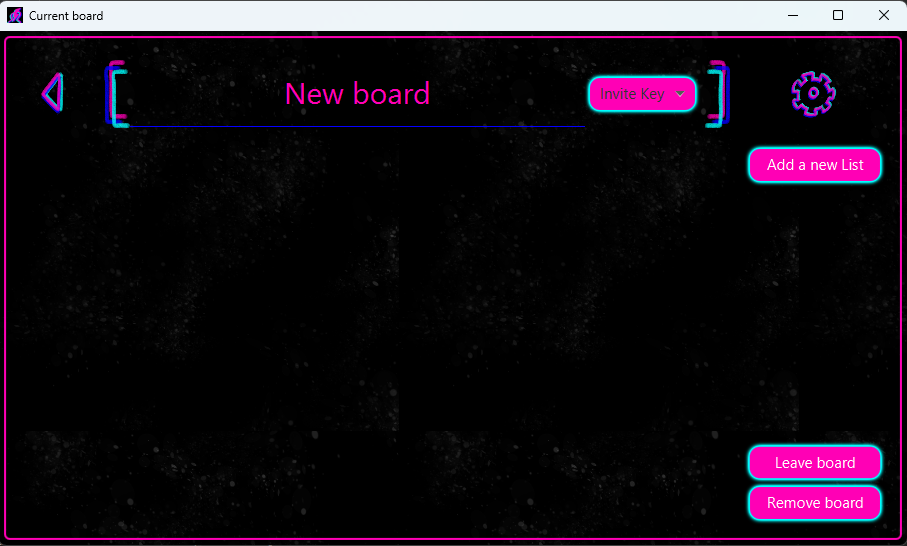
\includegraphics[scale=0.3]{boardoverview.png}
\caption{The board overview screen.}
\end{figure}

To access a board, a user first has to log on. The user can enter a username and the server IP on this screen. They can also claim admin access, and provide the admin password. Admins have access to all boards currently on the server, as opposed to users, who can only access boards if they have the invite key.

\begin{figure}[ht]
    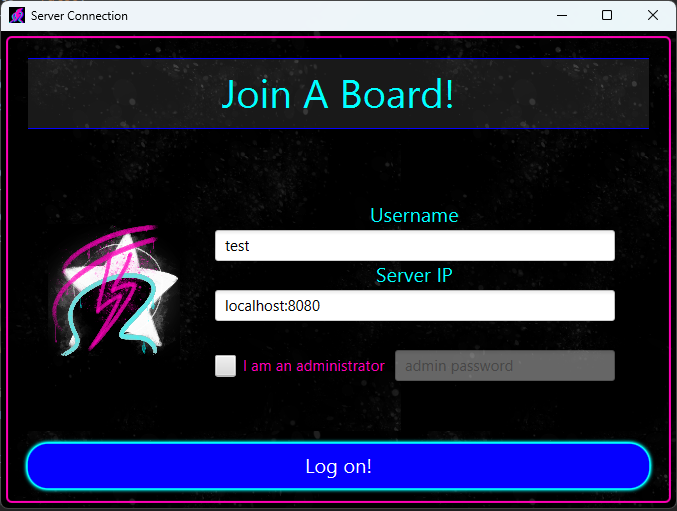
\includegraphics[scale=0.4]{logon.png}
    \caption{The logon screen.}
\end{figure}
 
 The boards can be accessed in parallel by all members of the board, using the board key. Users can also create new boards.

\begin{figure}[ht]
    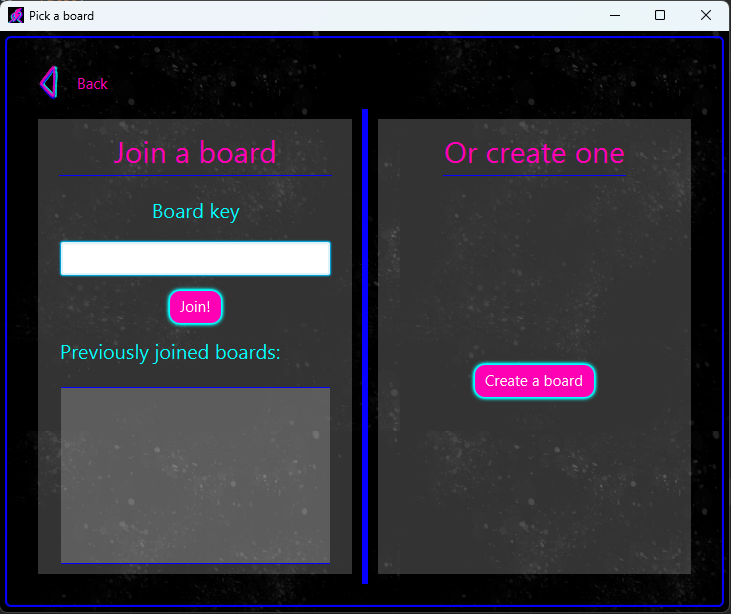
\includegraphics[scale=0.35]{boards.png}
    \caption{The boards screen.}
\end{figure}

In the board settings, a board can be renamed, and several customisation options exist to alter the appearance of a board. The board can also have tags, which then become accessible to all cards of the board. Users can also choose to leave or delete boards if they so wish.

\begin{figure}[ht]
    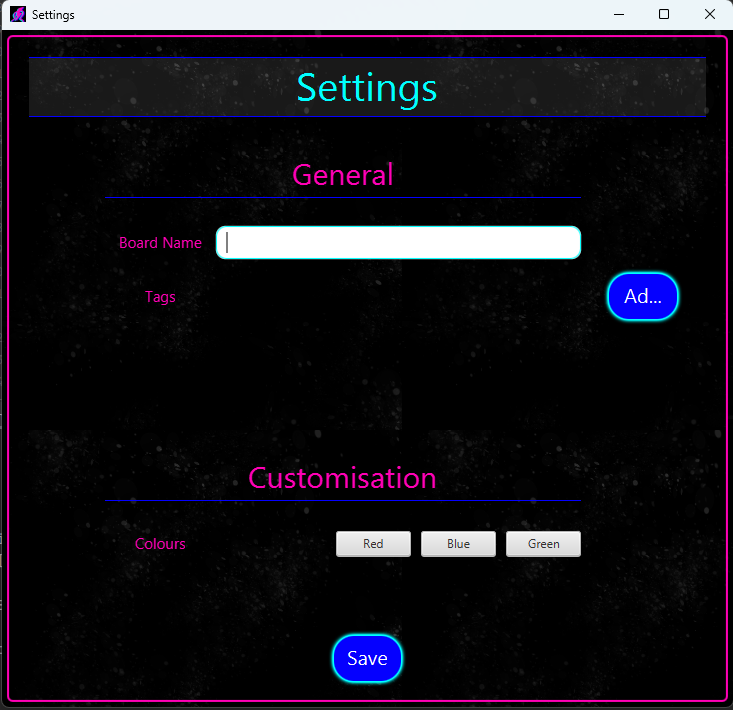
\includegraphics[scale=0.3]{settings.png}
    \caption{The settings screen.}
\end{figure}

When double-clicking on a specific card, a user can edit its title, tags, description, and subtasks.

\begin{figure}[ht]
    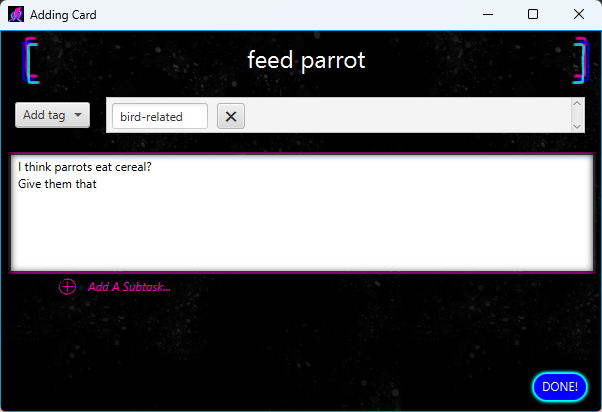
\includegraphics[scale=0.3]{carddetails.png}
    \caption{The card details screen.}
\end{figure}

The GUI design of the board seeks to emulate a blackboard, with a black background and a high-contrast, bright colour palette. The UI can also be interacted with without use of the mouse, as all elements are traverse-able using the TAB key. Generous highlighting and error pop-ups provide the user with instant visual feedback on their actions. 
